\documentclass[11pt,a4paper]{article}
\usepackage[utf8]{inputenc}
\usepackage[T1]{fontenc}
\usepackage[french]{babel}
\usepackage[margin=2.5cm]{geometry}
\usepackage{graphicx}
\usepackage{hyperref}
\usepackage{amsmath}
\usepackage{booktabs}
\usepackage{xcolor}

\title{
    \vspace{-2cm}
    \textbf{Rapport de Projet Individuel : Reinforcement Learning}\\
    \Large Deep Q-Learning sur Autoroute : Parallélisation et Robustesse à la Densité
}
\author{Antoine Yezou}
\date{\today}

\begin{document}

\maketitle

\section{Ce que j'ai implémenté ou analysé}

Mes contributions se sont concentrées sur deux axes principaux : l'optimisation de notre infrastructure d'entraînement pour passer à l'échelle, et le développement de l'\textbf{Extension Task}, visant à analyser et améliorer la robustesse de l'agent face aux variations de densité du trafic.

\paragraph{1. Pipeline d'entraînement parallélisé :} 
L'entraînement classique d'un DQN est souvent très gourmand en échantillons. Sur un environnement limité par le CPU comme \texttt{highway-env}, c'est particulièrement long. Pour contourner ce problème, j'ai mis en place une architecture d'entraînement parallélisée avec \texttt{SubprocVecEnv} (Stable Baselines 3). J'ai adapté notre boucle \texttt{train\_dqn} pour supporter l'inférence GPU par batch sur plusieurs environnements en même temps. En collectant les transitions de manière asynchrone depuis plusieurs workers (généralement autant que de cœurs CPU), ce pipeline permet un entraînement \textbf{environ 10 fois plus rapide} que la version séquentielle de base. Cela nous a permis d'itérer beaucoup plus vite sur les hyperparamètres.

\paragraph{2. Framework de l'Extension Task (Robustesse à la densité) :} 
Nos premiers modèles ont tous été entraînés sur un environnement statique (densité fixée à $1.0$). J'ai fait l'hypothèse que l'agent risquait de faire de l'overfitting sur cette configuration exacte et qu'il échouerait probablement si on le plaçait sur une autoroute vide ou, au contraire, complètement bouchée. Pour vérifier cela, j'ai créé le script \texttt{robustness\_eval.py}, qui permet de tester systématiquement un agent pré-entraîné sur des données Out-Of-Distribution (OOD), avec des densités allant de $0.75$ à $4.0$. De plus, j'ai remarqué que la vitesse minimale de la tâche principale (Core Task) était fixée à 20, ce qui rendait physiquement impossible pour notre agent d'éviter certains crashs (surtout à forte densité). J'ai donc modifié la configuration de l'extension (\texttt{extension\_config.py}) pour rajouter des vitesses cibles plus faibles.

\paragraph{3. Entraînements robustes (\texttt{main\_robust.py}) :}
Pour corriger ces problèmes de robustesse, j'ai proposé de nouvelles architectures d'entraînement pour forcer l'agent à généraliser. J'ai implémenté trois Gym Wrappers :
\begin{itemize}
    \item \textbf{Domain Randomization (\texttt{RandomDensityWrapper}) :} La densité est choisie aléatoirement entre $[0.75, 3.0]$ au début de chaque épisode.
    \item \textbf{Curriculum Learning (\texttt{CurriculumDensityWrapper}) :} La difficulté augmente doucement, en faisant passer la densité de $0.5$ à $3.0$ au cours de l'entraînement.
    \item \textbf{Mixed Curriculum (\texttt{MixedDensityWrapper}) :} Un mix des deux méthodes pour éviter l'oubli catastrophique. On augmente la densité linéairement sur les 50 premiers pourcents de l'entraînement, puis on bascule sur de la sélection aléatoire (Domain Randomization).
\end{itemize}

\section{Les expériences menées}

Pour valider l'impact de ces modifications, j'ai lancé deux grandes séries d'expériences :
\begin{enumerate}
    \item \textbf{Baseline Benchmark :} J'ai évalué les modèles de base (SB3 DQN et notre DQN maison) sur différentes densités ($\in [0.75, 4.0]$). J'ai suivi des métriques concrètes comme le taux de crash, la reward moyenne, et les vitesses atteintes.
    \item \textbf{Comparaison des méthodes robustes :} Avec \texttt{main\_robust.py}, j'ai entraîné des agents sur les trois frameworks (Random, Curriculum, Mixed). Pour que le Curriculum fonctionne bien, j'ai développé un \texttt{CyclicEpsilonDQNAgent} qui relance l'exploration (remonte le epsilon) à chaque fois qu'on franchit un palier de difficulté. J'ai ensuite repassé ces agents dans le pipeline d'évaluation pour comparer leurs résultats en OOD face à l'agent classique.
\end{enumerate}

\section{Succès et limites rencontrées}

\paragraph{Ce qui a fonctionné :}
\begin{itemize}
    \item \textbf{L'accélération via la parallélisation :} Le multiprocessing avec les batchs a très bien marché. L'entraînement est beaucoup plus rapide sans perdre en stabilité.
    \item \textbf{L'approche "Mixed" :} C'est le meilleur compromis. L'agent apprend facilement les bases (changer de voie) quand la route est dégagée, et la phase de randomisation sur la fin l'empêche d'oublier ces réflexes tout en le forçant à gérer les embouteillages.
    \item \textbf{Les scripts d'évaluation automatisés :} \texttt{robustness\_eval.py} permet de générer de beaux graphes comparatifs sur la reward, le taux de crash et la vitesse, ce qui clarifie l'analyse.
\end{itemize}

\paragraph{Ce qui a échoué ou posé problème :}
\begin{itemize}
    \item \textbf{Nombre de steps initial trop faible :} Au début, en testant sur 25 000 steps, les agents robustes et normaux avaient des résultats très similaires en OOD. Un modèle exposé à des densités variées a besoin de beaucoup plus de temps pour généraliser. Il a fallu pousser les entraînements à plus de 100 000 steps pour voir une vraie différence.
    \item \textbf{Le "Catastrophic Forgetting" du Curriculum :} Le \texttt{CurriculumDensityWrapper} pur a été victime d'un oubli catastrophique flagrant. Une fois que l'agent savait naviguer dans les fortes densités ($3.0$), il avait totalement oublié comment accélérer correctement sur une autoroute vide ($0.75$), ce qui ruinait ses performances sur les environnements faciles.
\end{itemize}

\begin{figure}[htpb]
    \centering
    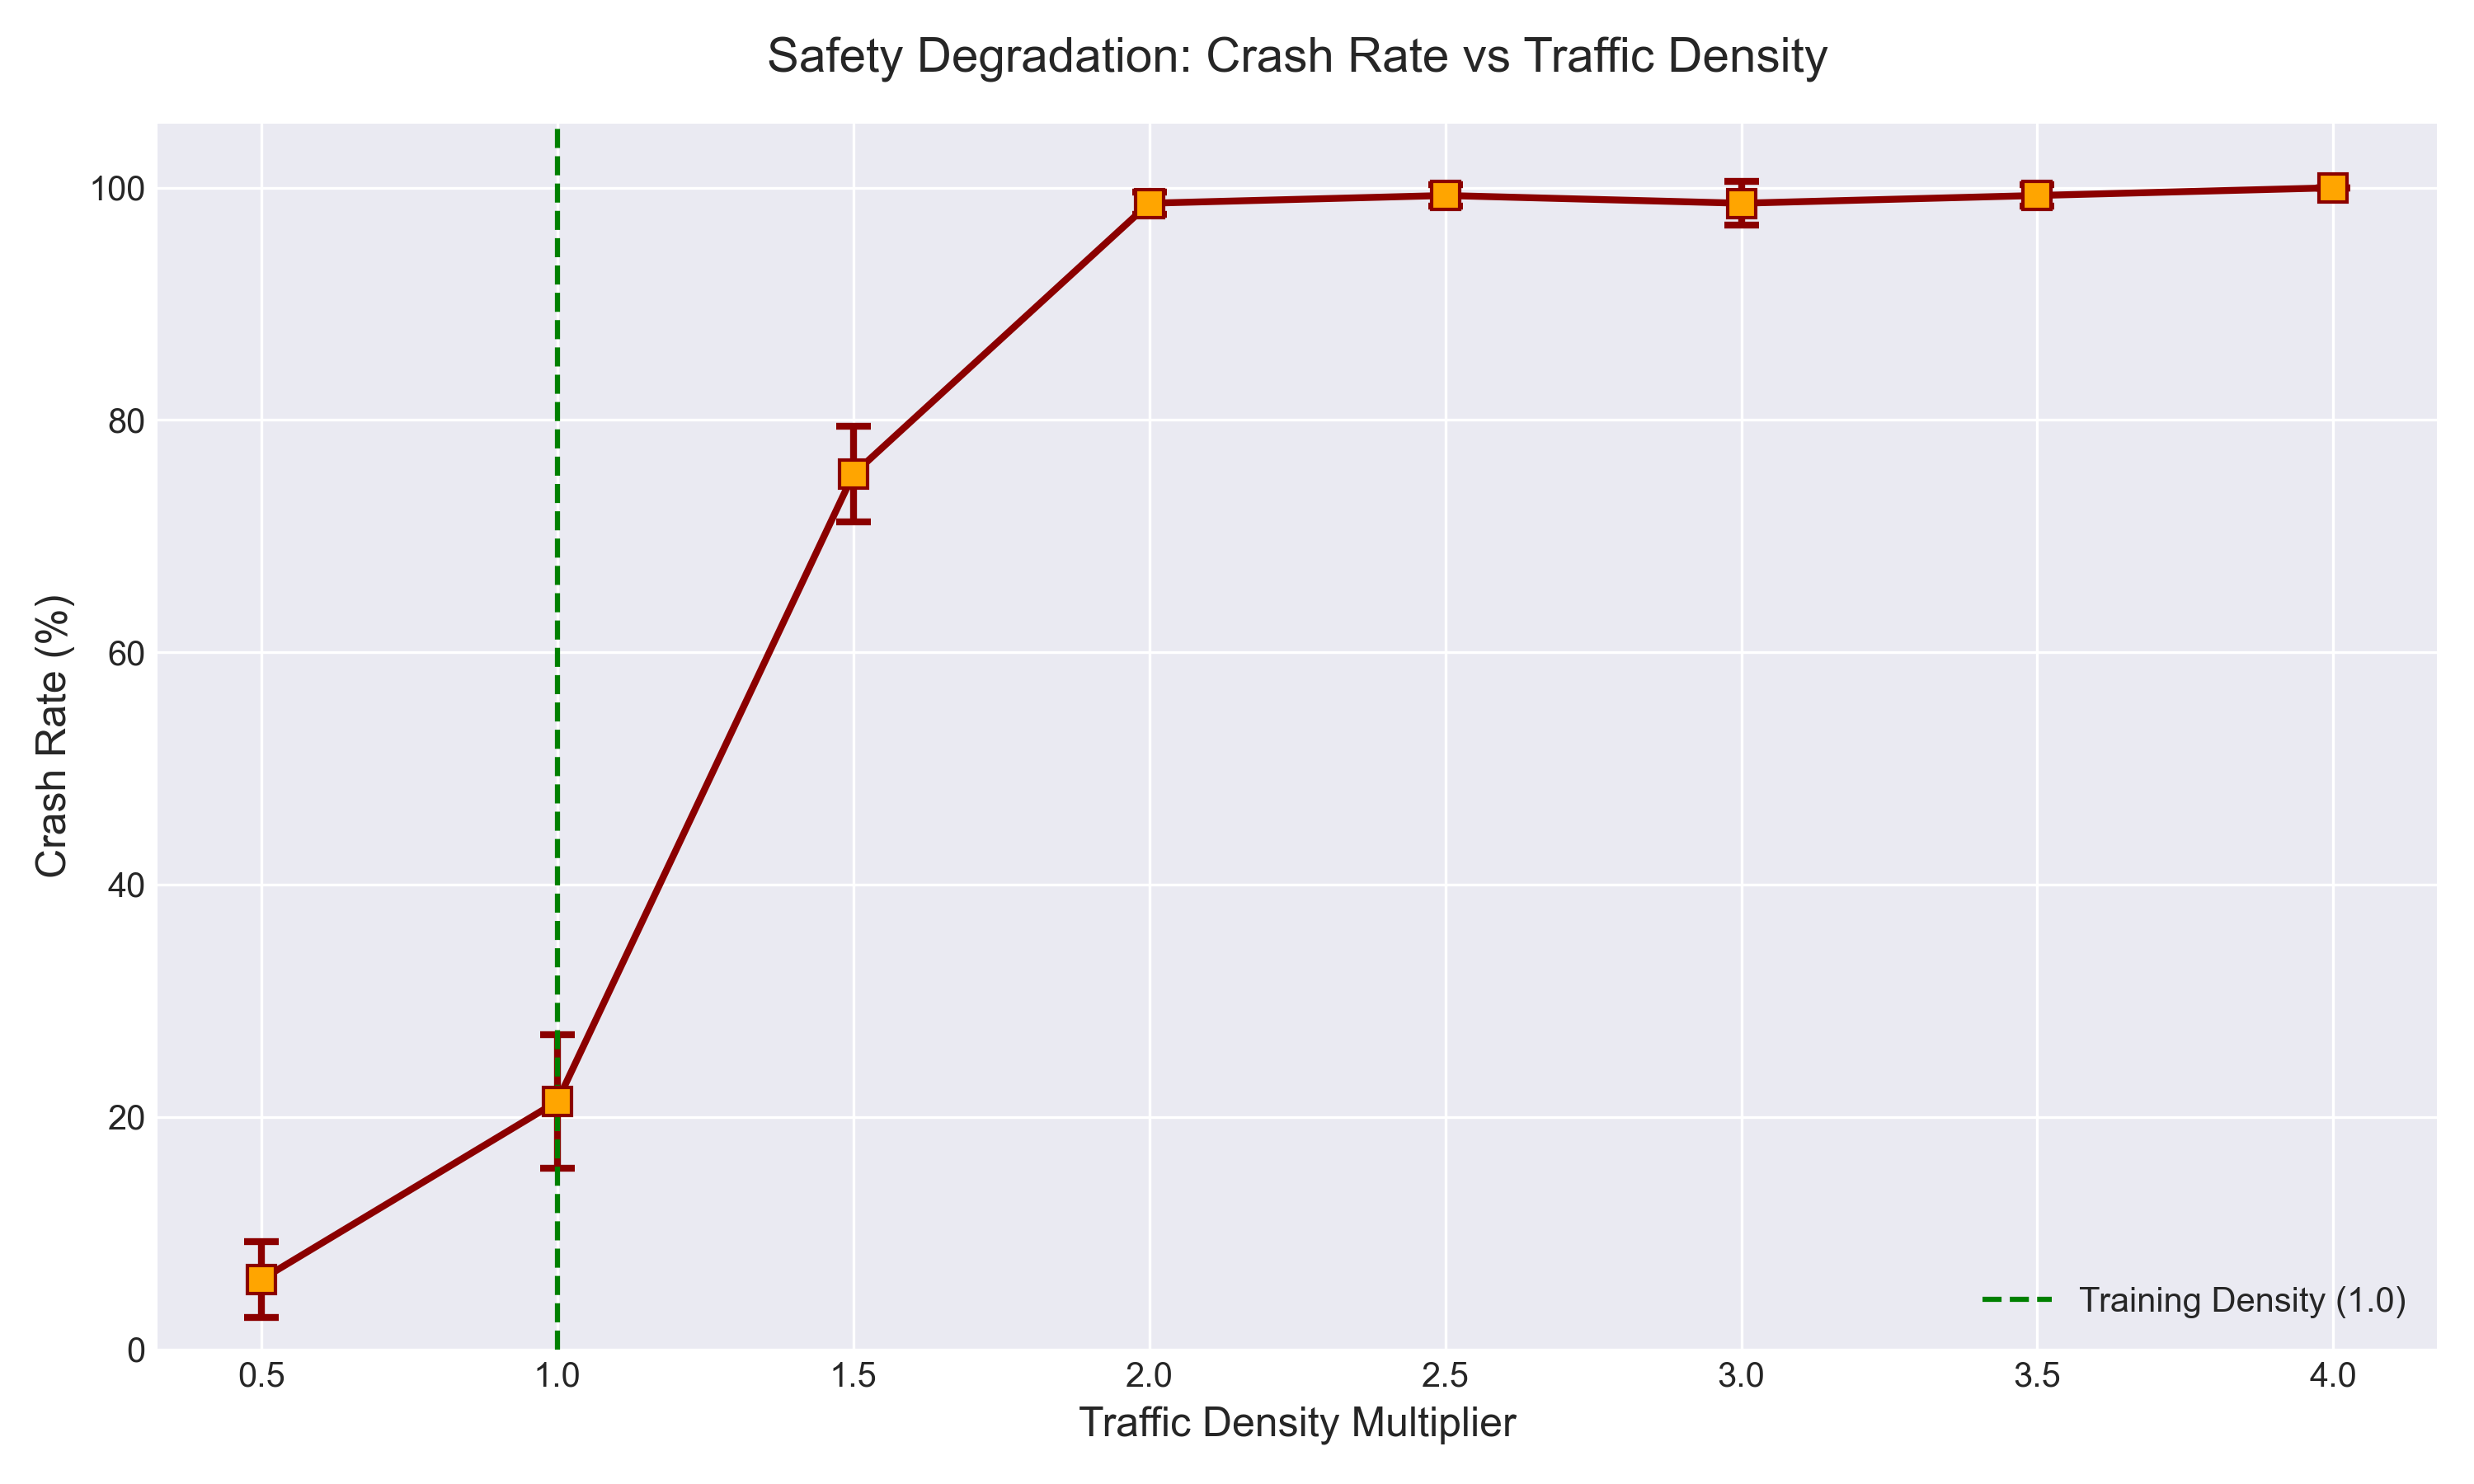
\includegraphics[width=0.75\textwidth]{../../results/figures/robustness_crash_rate_vs_density.png}
    \caption{Dégradation de la sécurité en OOD : Taux de crash vs Densité du trafic. On voit clairement que l'agent de base perd en fiabilité dès qu'on s'écarte de la densité d'entraînement.}
    \label{fig:crash_rate}
\end{figure}

\section{Preuves de contribution}

Toute la logique décrite ici est versionnée sur le repo du projet. Mon travail se retrouve principalement dans :
\begin{itemize}
    \item \texttt{core/dqn\_agent.py} : Implémentation du \texttt{train\_dqn\_parallel} pour la gestion asynchrone des workers et le batching GPU.
    \item \texttt{extension/robustness\_eval.py} : Le script d'évaluation OOD complet et sa logique de visualisation avec Matplotlib.
    \item \texttt{main\_robust.py} : Le développement du \texttt{CyclicEpsilonDQNAgent}, et des trois wrappers de densité (\texttt{Random}, \texttt{Curriculum}, et \texttt{Mixed}).
\end{itemize}

\section{Discussion sur les limites}

Si ces architectures robustes sont intéressantes, il reste quelques aspects à améliorer :
\begin{itemize}
    \item \textbf{Le réglage de l'Epsilon Cyclique :} Le reboot de l'exploration marche bien mais repose sur des heuristiques fixées à la main. Si on calibre mal les paliers de difficulté du curriculum, l'agent explore inutilement des situations qu'il maîtrise déjà.
    \item \textbf{Généralisation 1D plutôt que Multi-D :} Pour l'instant, on ne fait varier que la densité. Dans un vrai cadre de Sim2Real, un agent robuste devrait faire face à des variations simultanées (agressivité des conducteurs, friction du sol, bruit de capteurs, etc.). Projeter l'approche *Mixed* sur de multiples dimensions en même temps demanderait de revoir la méthode d'échantillonnage pour éviter que l'espace des états devienne intraitable (trop sparse) pour notre DQN actuel.
    \item \textbf{Des métriques centrées sur le crash :} On évalue surtout la robustesse via le taux d'accidents et la reward globale. Mais dans la réalité, un modèle "robuste" devrait aussi intégrer des notions de confort (limiter le jerk, les gros coups de frein) et de "politesse". Notre système a du mal à quantifier cela car \texttt{highway-env} distribue surtout des récompenses éparses liées au crash.
\end{itemize}

\end{document}